% Options for packages loaded elsewhere
\PassOptionsToPackage{unicode}{hyperref}
\PassOptionsToPackage{hyphens}{url}
%
\documentclass[
  ignorenonframetext,
]{beamer}
\usepackage{pgfpages}
\setbeamertemplate{caption}[numbered]
\setbeamertemplate{caption label separator}{: }
\setbeamercolor{caption name}{fg=normal text.fg}
\beamertemplatenavigationsymbolsempty
% Prevent slide breaks in the middle of a paragraph
\widowpenalties 1 10000
\raggedbottom
\setbeamertemplate{part page}{
  \centering
  \begin{beamercolorbox}[sep=16pt,center]{part title}
    \usebeamerfont{part title}\insertpart\par
  \end{beamercolorbox}
}
\setbeamertemplate{section page}{
  \centering
  \begin{beamercolorbox}[sep=12pt,center]{part title}
    \usebeamerfont{section title}\insertsection\par
  \end{beamercolorbox}
}
\setbeamertemplate{subsection page}{
  \centering
  \begin{beamercolorbox}[sep=8pt,center]{part title}
    \usebeamerfont{subsection title}\insertsubsection\par
  \end{beamercolorbox}
}
\AtBeginPart{
  \frame{\partpage}
}
\AtBeginSection{
  \ifbibliography
  \else
    \frame{\sectionpage}
  \fi
}
\AtBeginSubsection{
  \frame{\subsectionpage}
}
\usepackage{amsmath,amssymb}
\usepackage{lmodern}
\usepackage{ifxetex,ifluatex}
\ifnum 0\ifxetex 1\fi\ifluatex 1\fi=0 % if pdftex
  \usepackage[T1]{fontenc}
  \usepackage[utf8]{inputenc}
  \usepackage{textcomp} % provide euro and other symbols
\else % if luatex or xetex
  \usepackage{unicode-math}
  \defaultfontfeatures{Scale=MatchLowercase}
  \defaultfontfeatures[\rmfamily]{Ligatures=TeX,Scale=1}
\fi
% Use upquote if available, for straight quotes in verbatim environments
\IfFileExists{upquote.sty}{\usepackage{upquote}}{}
\IfFileExists{microtype.sty}{% use microtype if available
  \usepackage[]{microtype}
  \UseMicrotypeSet[protrusion]{basicmath} % disable protrusion for tt fonts
}{}
\makeatletter
\@ifundefined{KOMAClassName}{% if non-KOMA class
  \IfFileExists{parskip.sty}{%
    \usepackage{parskip}
  }{% else
    \setlength{\parindent}{0pt}
    \setlength{\parskip}{6pt plus 2pt minus 1pt}}
}{% if KOMA class
  \KOMAoptions{parskip=half}}
\makeatother
\usepackage{xcolor}
\IfFileExists{xurl.sty}{\usepackage{xurl}}{} % add URL line breaks if available
\IfFileExists{bookmark.sty}{\usepackage{bookmark}}{\usepackage{hyperref}}
\hypersetup{
  pdftitle={vizcovidfr, a Covid-19 analysis package},
  pdfauthor={Amélie Vernay, Laurent Llinares, Quentin Foux, Alexandre Nicolas},
  hidelinks,
  pdfcreator={LaTeX via pandoc}}
\urlstyle{same} % disable monospaced font for URLs
\newif\ifbibliography
\usepackage{longtable,booktabs,array}
\usepackage{calc} % for calculating minipage widths
\usepackage{caption}
% Make caption package work with longtable
\makeatletter
\def\fnum@table{\tablename~\thetable}
\makeatother
\usepackage{graphicx}
\makeatletter
\def\maxwidth{\ifdim\Gin@nat@width>\linewidth\linewidth\else\Gin@nat@width\fi}
\def\maxheight{\ifdim\Gin@nat@height>\textheight\textheight\else\Gin@nat@height\fi}
\makeatother
% Scale images if necessary, so that they will not overflow the page
% margins by default, and it is still possible to overwrite the defaults
% using explicit options in \includegraphics[width, height, ...]{}
\setkeys{Gin}{width=\maxwidth,height=\maxheight,keepaspectratio}
% Set default figure placement to htbp
\makeatletter
\def\fps@figure{htbp}
\makeatother
\setlength{\emergencystretch}{3em} % prevent overfull lines
\providecommand{\tightlist}{%
  \setlength{\itemsep}{0pt}\setlength{\parskip}{0pt}}
\setcounter{secnumdepth}{-\maxdimen} % remove section numbering
\ifluatex
  \usepackage{selnolig}  % disable illegal ligatures
\fi

\title{vizcovidfr, a Covid-19 analysis package}
\author{Amélie Vernay, Laurent Llinares, Quentin Foux, Alexandre
Nicolas}
\date{25/04/2021}

\begin{document}
\frame{\titlepage}

\begin{frame}{Our goals}
\protect\hypertarget{our-goals}{}
\begin{itemize}
\tightlist
\item
  Analyze the spreading of the Covid-19 disease in France. \pause
\item
  Produce various charts to illustrate how the Covid-19 affects
  population. \pause
\item
  Predict how the Covid-19 will evolve in the future. \pause
\item
  Create a simple visualization tool as interactive as possible and easy
  to use for anyone.
\end{itemize}
\end{frame}

\begin{frame}{Data (part 1/3)}
\protect\hypertarget{data-part-13}{}
\begin{itemize}
\tightlist
\item
  All the datasets that we used are taken from
  \url{https://www.data.gouv.fr/fr/pages/donnees-coronavirus}. \pause
\item
  Data is collected almost every day per region / department for
  different variables such as hospitalization or death for example.
  \pause
\item
  Here is a summary table of every dataset used. \pause
\end{itemize}
\end{frame}

\begin{frame}[fragile]{Data (part 2/3)}
\protect\hypertarget{data-part-23}{}
\begin{longtable}[]{@{}
  >{\centering\arraybackslash}p{(\columnwidth - 2\tabcolsep) * \real{0.36}}
  >{\centering\arraybackslash}p{(\columnwidth - 2\tabcolsep) * \real{0.64}}@{}}
\toprule
dataset & desciption \\
\midrule
\endhead
\texttt{chiffres-cles} & hospitalization, intensive care, death, by
regions and departments \\
\texttt{chiffres-fr} & cases, hospitalization, intensive care, death for
the whole France \\
\texttt{classe\_age} & hospitalization, intensive care, death, by age
range and region \\
\texttt{covid-19-france-vaccinations-age-dep} & vaccine administration
by age \\
\texttt{stocks-es-national} & vaccine type in storage \\
\texttt{transfer.csv} & patient transfers \\
\bottomrule
\end{longtable}
\end{frame}

\begin{frame}[fragile]{Data (part 3/3)}
\protect\hypertarget{data-part-33}{}
\begin{longtable}[]{@{}
  >{\centering\arraybackslash}p{(\columnwidth - 2\tabcolsep) * \real{0.37}}
  >{\centering\arraybackslash}p{(\columnwidth - 2\tabcolsep) * \real{0.63}}@{}}
\toprule
dataset & desciption \\
\midrule
\endhead
\texttt{posquotreg} & positivity and tests by sex and age for regions
(daily) \\
\texttt{posquotfr} & positivity and tests by sex and age for the whole
France (daily) \\
\texttt{poshebreg} & positivity and tests by sex and age for regions
(weekly) \\
\texttt{poshebfr} & positivity and tests by sex and age for the whole
France (weekly) \\
\texttt{incquotreg} & incidence rate by sex and age for regions \\
\texttt{incquotfr} & incidence rate by sex and age for the whole
France \\
\bottomrule
\end{longtable}
\end{frame}

\begin{frame}[fragile]{Module structure (part 1/3)}
\protect\hypertarget{module-structure-part-13}{}
\begin{verbatim}
vizcovidfr
|   .github/workflows
|   beamer
|   doc
│   report
|   vizcovidfr
|   .gitignore
|   README.md
|   requirements.txt
└── setup.py
\end{verbatim}
\end{frame}

\begin{frame}[fragile]{Module structure (part 2/3)}
\protect\hypertarget{module-structure-part-23}{}
\begin{verbatim}
vizcovidfr
|   ...
│
└───vizcovidfr
│   │   barplots
│   │   data
|   |   heatmap
|   |   line_charts
|   |   loads
|   |   maps
|   |   pie_charts
|   |   prediction
|   |   preprocesses
|   |   regression
|   |   sparse
|   |   tests
|   |   README.md
|   └── __init__.py
│
└───...
\end{verbatim}
\end{frame}

\begin{frame}[fragile]{Module structure (part 3/3)}
\protect\hypertarget{module-structure-part-33}{}
\begin{verbatim}
vizcovidfr
|   ...
│
└───vizcovidfr
│   │   ...
|   |
│   └───tests
│       │   __init__.py
│       └── test_vizcovidfr.py
|
│
└───...
\end{verbatim}
\end{frame}

\begin{frame}[fragile]{\texttt{test\_vizcovidfr.py}}
\protect\hypertarget{test_vizcovidfr.py}{}
\begin{verbatim}
def test_viz3Dmap():
    """
    Test viz3Dmap by running the function.
    If something fails while running it, result won't be defined,
    and an AssertionError will raise.
    ---
    Functions/methods that will be tested by extension:
        - load_datasets.Load_chiffres_cles().save_as_df()
        - preprocess_chiffres_cles.drop_some_columns()
        - preprocess_chiffres_cles.reg_depts()
        - preprocess_chiffres_cles.reg_depts_code_format()
        - preprocess_maps.map_save_path_routine()
    """
    result = (type(maps.viz3Dmap(file_path='')) != int)
    assert
\end{verbatim}
\end{frame}

\begin{frame}{Workflow}
\protect\hypertarget{workflow}{}
\begin{itemize}
\tightlist
\item
  Each contributor created a class to load the dataset he used. \pause
\item
  Each contributor put as many functions as possible in preprocess to
  have a clear code, which allowed others to use them. \pause
\item
  Each contributor worked on his branch to avoid conflicts. \pause
\item
  Each contributor created his own modules, with its documentation and
  their unit tests associated.
\end{itemize}
\end{frame}

\begin{frame}{Regression and prediction (part 1/6)}
\protect\hypertarget{regression-and-prediction-part-16}{}
\begin{itemize}
\tightlist
\item
  Because we had data relative to the time, we wanted to predict the
  evolution of Covid-19. \pause Here is an example of scatter plot
  \pause \includegraphics{scatter_hospitalization_Île-de-France.pdf}
\end{itemize}
\end{frame}

\begin{frame}{Regression and prediction (part 2/6)}
\protect\hypertarget{regression-and-prediction-part-26}{}
Linear regression is not adapted to data. \pause How to make prediction
then ? \pause \(\implies\) Polynomial regression

Pros and cons :

\begin{itemize}
\tightlist
\item
  Curve predicted follows well the data. \pause
\item
  Regression has a good R2 (lots of models have more than \(90 \%\)).
  \pause
\item
  Good prediction of foreseeable future. \pause
\item
  Problem : impossible to predict in a far future
\end{itemize}
\end{frame}

\begin{frame}{Regression and prediction (part 3/6)}
\protect\hypertarget{regression-and-prediction-part-36}{}
\begin{figure}
\centering
\includegraphics{regression_hospitalization_Île-de-France.pdf}
\caption{Caption for the picture.}
\end{figure}
\end{frame}

\begin{frame}{Regression and prediction (part 4/6)}
\protect\hypertarget{regression-and-prediction-part-46}{}
Prediction for 2021-04-30 (with data until 2021-04-23) :

\begin{figure}
\centering
\includegraphics{predict_hospitalization_Île-de-France_2021-04-30.pdf}
\caption{Caption for the picture.}
\end{figure}
\end{frame}

\begin{frame}{Regression and prediction (part 5/6)}
\protect\hypertarget{regression-and-prediction-part-56}{}
Prediction for 2021-06-30 (with data until 2021-04-23) :

\begin{figure}
\centering
\includegraphics{predict_hospitalization_Île-de-France_2021-06-30.pdf}
\caption{Caption for the picture.}
\end{figure}
\end{frame}

\begin{frame}{Regression and prediction (part 6/6)}
\protect\hypertarget{regression-and-prediction-part-66}{}
Advice :

\begin{itemize}
\tightlist
\item
  Use first poly\_fit function to see how the model fits with data.
  \pause
\item
  Then use predict\_curve to check if the predicted curve is going to
  infinite or not. \pause
\item
  If predicted curve looks good, then use predict\_value to get the
  value you were looking for.
\end{itemize}
\end{frame}

\begin{frame}{Time and memory}
\protect\hypertarget{time-and-memory}{}
\begin{itemize}
\tightlist
\item
  Each function displays its execution time and they're all calculated
  on the same machine. \pause
\item
  Proportionality between dataset size and execution time (the bigger
  the dataset is, the longer it will be loaded). \pause
\end{itemize}
\end{frame}

\begin{frame}{Conclusion / Doorway / Examples}
\protect\hypertarget{conclusion-doorway-examples}{}
\begin{itemize}
\tightlist
\item
  Watch the documentation to get thorough information about vizcovidfr's
  functions. \pause
\item
  Here are some examples taken from our notebook (in `report') to
  inspire you ! \pause 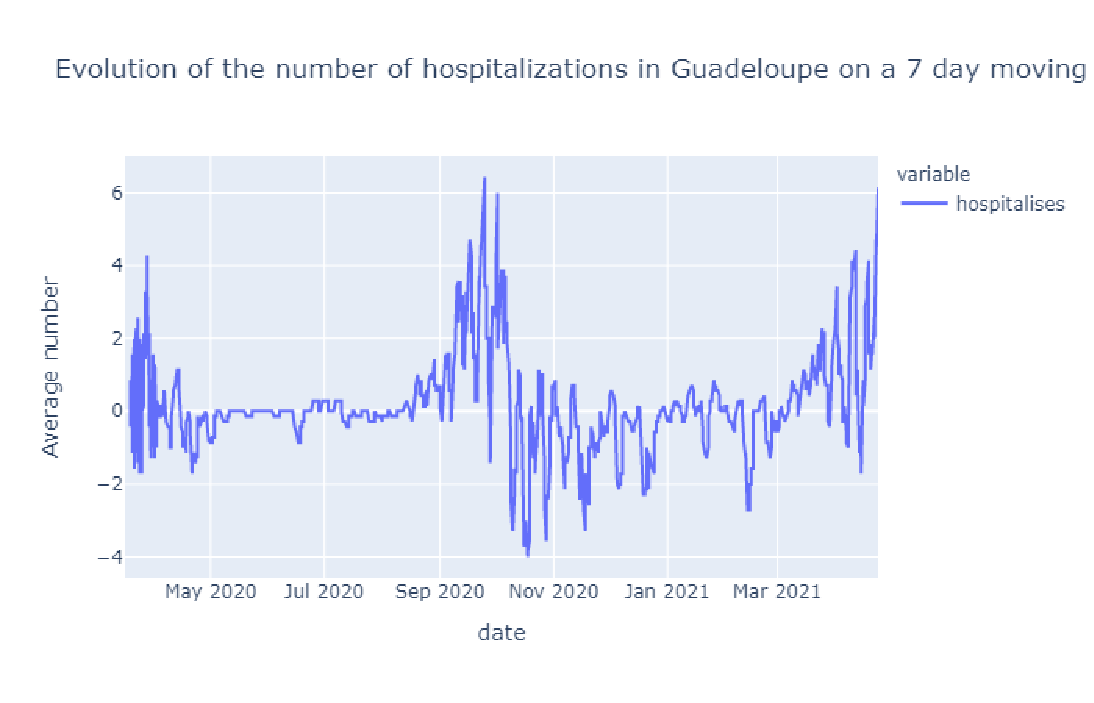
\includegraphics{line_chart_guadeloupe_hosp.pdf}
\end{itemize}
\end{frame}

\begin{frame}{Conclusion / Doorway / Examples}
\protect\hypertarget{conclusion-doorway-examples-1}{}
\begin{figure}
\centering
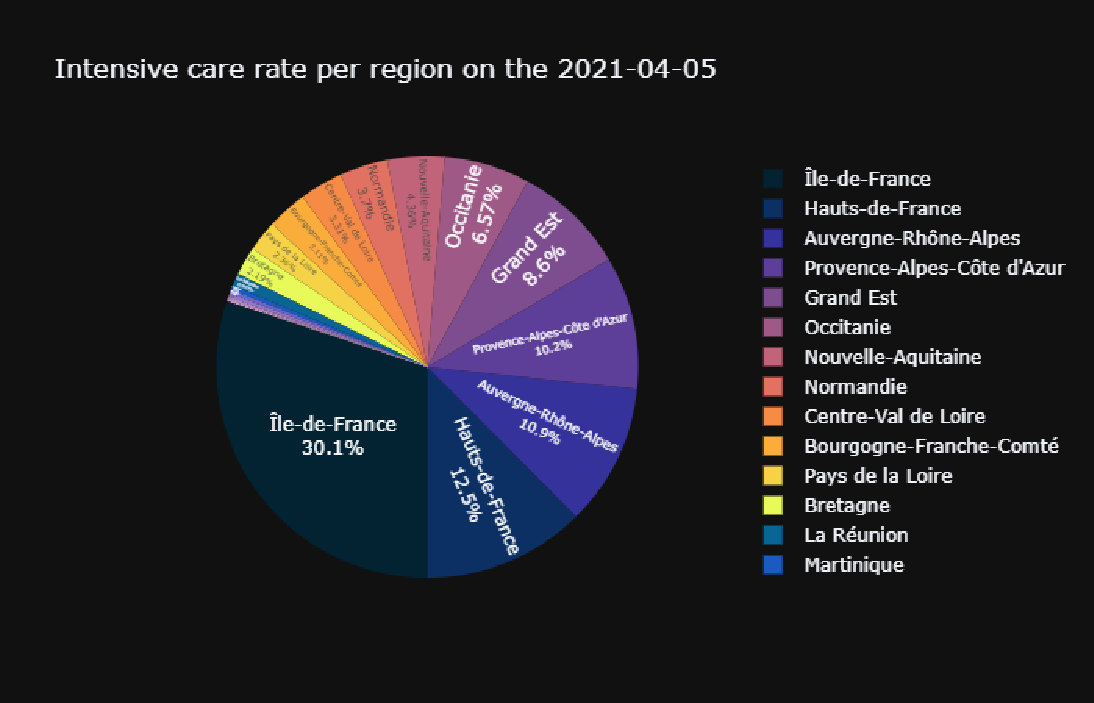
\includegraphics{piechart.pdf}
\caption{Caption for the picture.}
\end{figure}
\end{frame}

\begin{frame}{Conclusion / Doorway / Examples}
\protect\hypertarget{conclusion-doorway-examples-2}{}
\begin{figure}
\centering
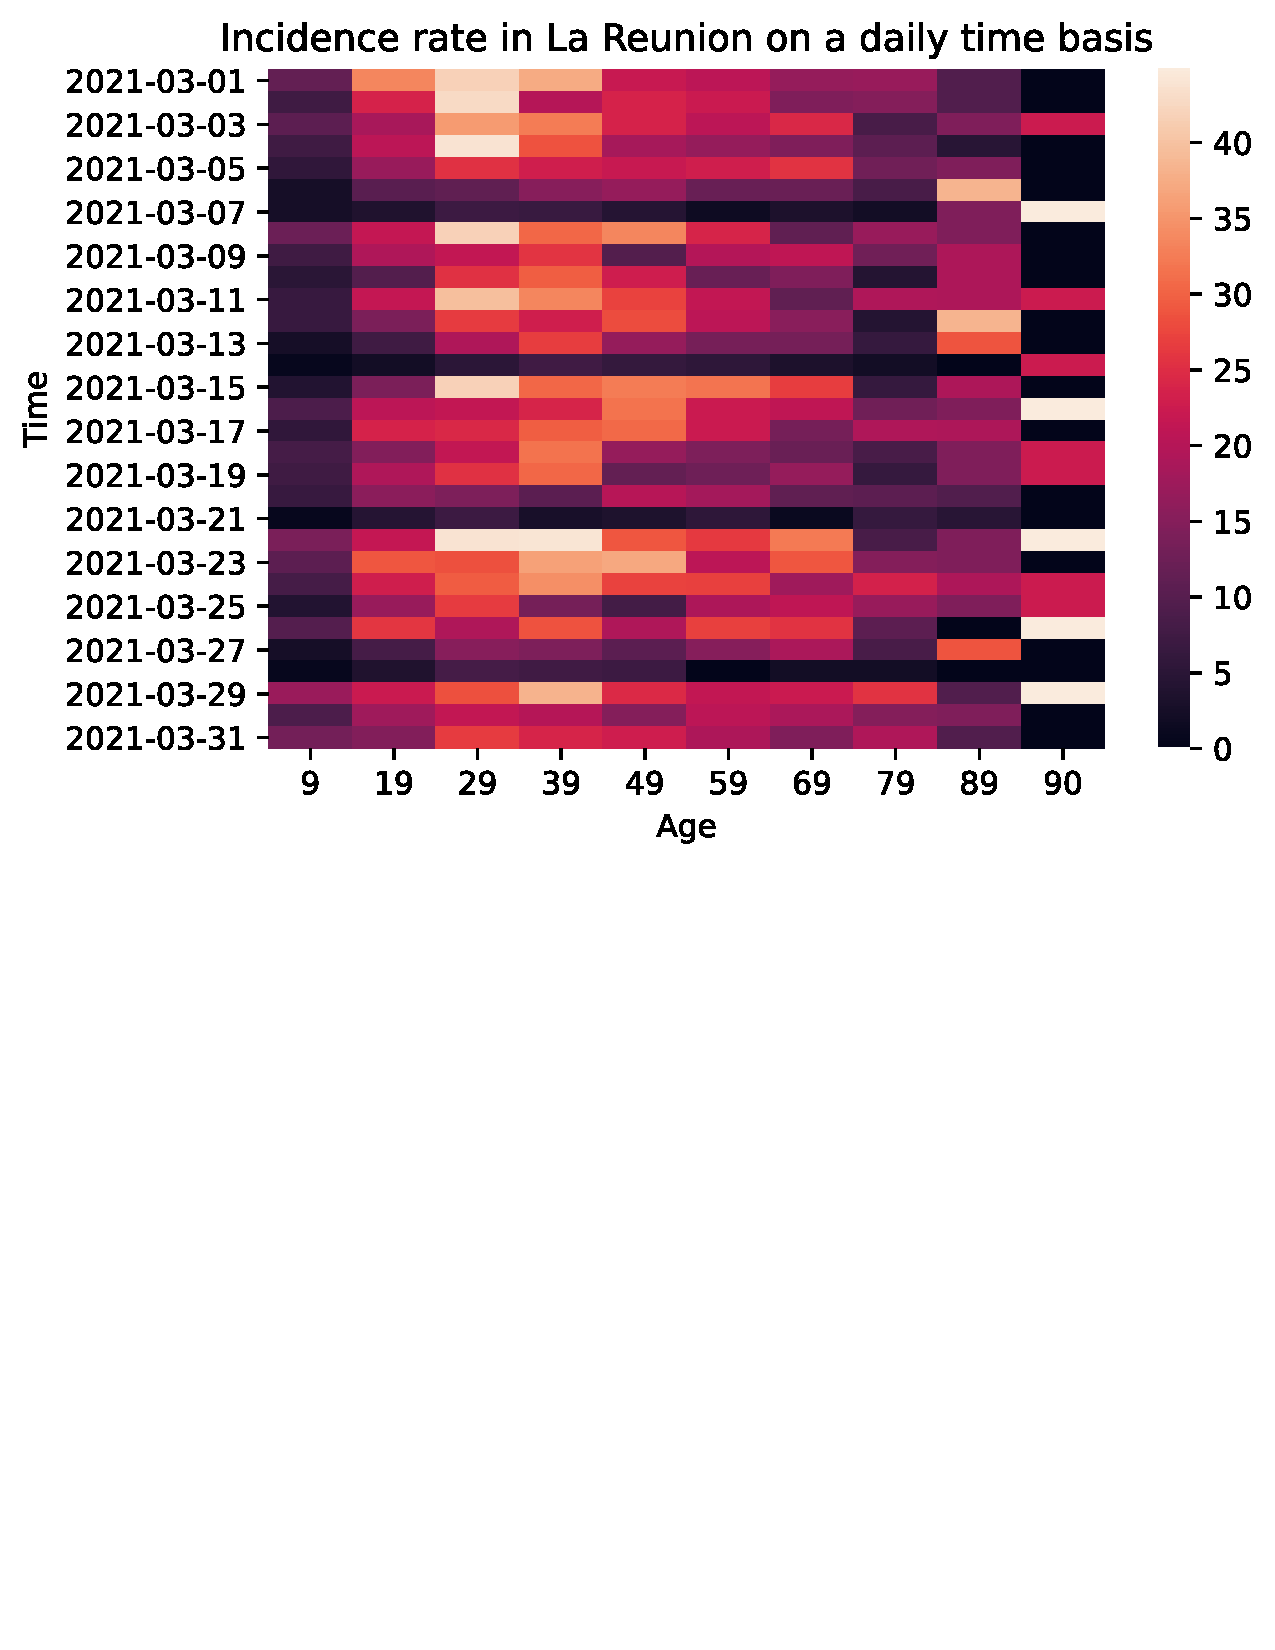
\includegraphics{heatmap_la_reunion_day.pdf}
\caption{Caption for the picture.}
\end{figure}
\end{frame}

\begin{frame}{Conclusion / Doorway / Examples}
\protect\hypertarget{conclusion-doorway-examples-3}{}
SPARSE
\end{frame}

\end{document}
